\documentclass{article}
\usepackage{tikz}
\usepackage{bm}
\newcommand{\vv}[1]{\bm{#1}}
\begin{document}
\begin{center}
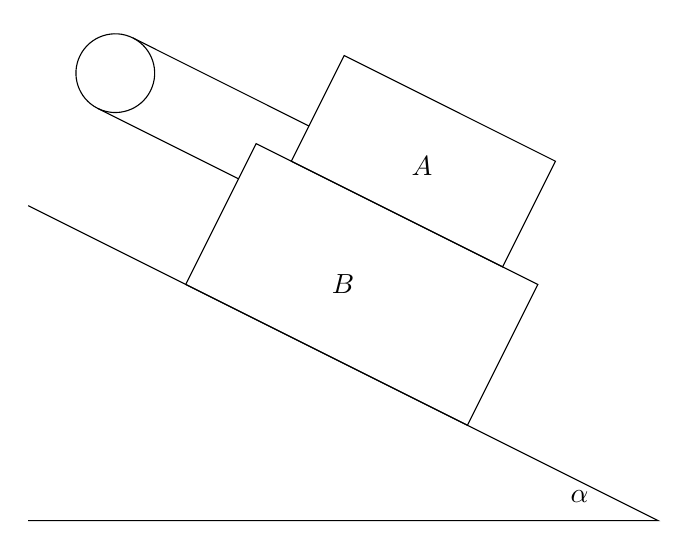
\begin{tikzpicture}
\draw (-4,0) -- (4,0) -- (-4,4);
\draw [rotate around={-26.57:(-2,3)}](-2,3) rectangle (2, 5);
\draw [rotate around={-26.57:(-2,3)}](-1.5,5) rectangle (1.5,6.5);
\draw [rotate around={-26.57:(-2,3)}](-4,5) circle [radius=0.5];
\draw [rotate around={-26.57:(-2,3)}](-4,5.5) -- (-1.5,5.5);
\draw [rotate around={-26.57:(-2,3)}](-4,4.5) -- (-2,4.5);
\node at (0,3) {\(B\)};
\node at (1,4.5) {\(A\)};
\node at (3,0.3) {\(\alpha\)};
\end{tikzpicture}

~\\

~\\

~\\

\begin{tikzpicture}
\draw [dotted] (-4,0) -- (4,0) -- (-4,4);
\draw [rotate around={-26.57:(-2,3)},dotted](-2,3) rectangle (2, 5);
\draw [rotate around={-26.57:(-2,3)}](-1.5,5) rectangle (1.5,6.5);
\draw [rotate around={-26.57:(-2,3)},dotted](-4,5) circle [radius=0.5];
\draw [rotate around={-26.57:(-2,3)},dotted](-4,5.5) -- (-1.5,5.5);
\draw [rotate around={-26.57:(-2,3)},dotted](-4,4.5) -- (-2,4.5);
\node at (1.7,4.3) {\(A\)};
\draw [rotate around={-26.57:(-2,3)}][->] (0,5) -- (0,7);
\draw [rotate around={-26.57:(-2,3)}][->] (0,5) -- (2.5,5);
\draw [rotate around={-26.57:(-2,3)}][->] (-1.5,5.5) -- (-2.5,5.5);
\draw [rotate around={-26.57:(-2,3)}][->] (3,7.5) -- (2,7.5);
\draw [rotate around={-26.57:(-2,3)}][<->] (3,6) -- (4,6) -- (4,7);
\node [above] at (-1.3,5.5) {\(\vv T_A\)};
\node [above] at (1.6,5.7) {\(\vv N_A\)};
\node [above] at (2.9,2.8) {\(\vv f_A\)};
\node [left] at (3.8,3.5) {\(\vv x\)};
\node [above] at (5.2,3.9) {\(\vv y\)};
\draw [->] (1,4.5) -- (1,3.3);
\node [below] at (1,3.3) {\(m\vv g\)};
\node [left] at (3.6,5.3) {\(\vv v_A\)};
\end{tikzpicture}

~\\

~\\

~\\

\begin{tikzpicture}
\draw [dotted](-4,0) -- (4,0) -- (-4,4);
\draw [rotate around={-26.57:(-2,3)}](-2,3) rectangle (2, 5);
\draw [rotate around={-26.57:(-2,3)},dotted](-1.5,5) rectangle (1.5,6.5);
\draw [rotate around={-26.57:(-2,3)},dotted](-4,5) circle [radius=0.5];
\draw [rotate around={-26.57:(-2,3)},dotted](-4,5.5) -- (-1.5,5.5);
\draw [rotate around={-26.57:(-2,3)},dotted](-4,4.5) -- (-2,4.5);
\node at (1,2.5) {\(B\)};
\draw [rotate around={-26.57:(-2,3)}][->] (0,3) -- (0,5.75);
\draw [rotate around={-26.57:(-2,3)}][->] (0,3) -- (-3,3);
\draw [rotate around={-26.57:(-2,3)}][->] (-2,4.5) -- (-3,4.5);
\draw [rotate around={-26.57:(-2,3)}][->] (-1,5) -- (-1,4);
\draw [rotate around={-26.57:(-2,3)}][->] (-1,5) -- (-3,5);
\node [above] at (-2.9,3.4) {\(\vv f_B\)};
\node [below] at (-2.2,4.7) {\(\vv T_B\)};
\node [above] at (-2,5.2) {\(-\vv f_A\)};
\node [right] at (0.8,4.7) {\(\vv N_B\)};
\node [below] at (-0.7,3.4) {\(-\vv N_A\)};
\draw [rotate around={-26.57:(-2,3)}][->] (2,7.5) -- (3,7.5);
\draw [rotate around={-26.57:(-2,3)}][<->] (5,6) -- (4,6) -- (4,7);
\draw [->] (0.245,3) -- (0.245,1);
\node [below] at (0.245,1) {\(M\vv g\)};
\node [right] at (4.4,4.8) {\(\vv v_B\)};
\node [above] at (5.2,3.9) {\(\vv y\)};
\node [right] at (5.6,2.5) {\(\vv x\)};
\end{tikzpicture}

~\\

~\\

~\\

\begin{tikzpicture}
\draw [dotted](-4,0) -- (4,0) -- (-4,4);
\draw [dotted][rotate around={-26.57:(-2,3)}](-2,3) rectangle (2, 5);
\draw [dotted][rotate around={-26.57:(-2,3)}](-1.5,5) rectangle (1.5,6.5);
\draw [rotate around={-26.57:(-2,3)}](-4,5) circle [radius=0.5];
\draw [rotate around={-26.57:(-2,3)}](-4,5.5) -- (-1.5,5.5);
\draw [rotate around={-26.57:(-2,3)}](-4,4.5) -- (-2,4.5);
\draw [rotate around={-26.57:(-2,3)}][->] (-4,4.5) -- (-3,4.5);
\draw [rotate around={-26.57:(-2,3)}][->] (-4,5.5) -- (-3,5.5);
\node [above] at (-1.8,5.7) {\(-\vv T_A\)};
\node [below] at (-2.3,4.8) {\(-\vv T_B\)};
\end{tikzpicture}

~\\

~\\

~\\

\begin{tikzpicture}
\draw [dotted](-4,0) -- (4,0) -- (-4,4);
\draw [rotate around={-26.57:(-2,3)}][dotted](-2,3) rectangle (2, 5);
\draw [rotate around={-26.57:(-2,3)}][dotted](-1.5,5) rectangle (1.5,6.5);
\draw [rotate around={-26.57:(-2,3)}](-4,5) circle [radius=0.5];
\draw [rotate around={-26.57:(-2,3)}](-4,5.5) -- (-1.5,5.5);
\draw [rotate around={-26.57:(-2,3)}](-4,4.5) -- (-2,4.5);
\draw [rotate around={-26.57:(-2,3)}][dashed, thick] (-2,4.5) -- (-2,3);
\draw [rotate around={-26.57:(-2,3)}][dashed, thick] (-1.5,5.5) -- (-1.5,3);
\draw [rotate around={-26.57:(-2,3)}][->] (-4,3) -- (3,3);
\node [below] at (-2,3) {\(x_B\)};
\node [below] at (-1.6,2.8) {\(x_a\)};
\draw [rotate around={-26.57:(-2,3)}][|-|](-4,4.4) arc [start angle = 270, end angle = 90, radius = 0.6];
\node at (-3.55,6) {\(l\)};
\draw [rotate around={-26.57:(-2,3)}][dashed,thick] (-4,4.5) -- (-4,3);
\node [below] at (-3.8, 3.9) {\(0\)};
\end{tikzpicture}
\end{center}
\end{document}